\section{Results}

\begin{frame}{During the Experiment} % _________________________________________
  \vspace{-0.15in}
  \hspace*{-12.5mm}
  \includegraphics[width=1.2\textwidth]<1>{../figures/results_run1.pdf}
  \includegraphics[width=1.2\textwidth]<2>
    {../figures/results_run2_novel_portion.png}
  \includegraphics[width=1.2\textwidth]<3>{../figures/results_run2.pdf}
  \includegraphics[width=1.2\textwidth]<4>{../figures/results_run3.pdf}

  \note<1>{\begin{itemize}
    \item Input - \ref{fig:run1}(d) shows the depth image $D$ generated from the
    simulated sensor. \ref{fig:run1}(a) shows us two important aspects to consider
    about $D$. First, the pose $P$ of the sensor is shown by looking at the
    sensor's view frustum, indicated by the blue wireframe. Second, the only
    environmental information used to generate the depth image is shown in light
    gray.
    \item Generate Expected Depth Image ($E$) - \ref{fig:run1}(e) shows the
    expected depth image $E$. \ref{fig:run1}(a) also shows us two important
    aspects to consider about $E$. First, the same pose $P$ is used to create both
    $D$ and $E$ (as indicated by the blue wire frame). Second, the only
    environmental information used to create $E$ is the yellow and light green
    parts of $M$ because that is the only information $M$ contains \emph{during}
    iteration 3.
    \item Classify Depth Image ($D$) - \ref{fig:run1}(f) visualizes the
    classification process. More specifically, it shows the points as expressed in
    Equation \ref{eqn:throwaway} in white ($D_{throwaway}$). \ref{fig:run1}(f) is
    important for understanding how MABDI works because it clearly shows which
    points will be thrown away (white) and which points will be kept for
    generating the novel surface $S$ (black).
    \item Surface Reconstruction - \ref{fig:run1}(b) shows the novel surface $S$
    in the context of the simulated environment. $S$ is constructed using all the
    points colored black in \ref{fig:run1}(f).
    \item Add Novel Surface ($S$) to Global Mesh($M$) - \ref{fig:run1}(a) shows
    the novel surface $S$ appended to the global mesh $M$ in dark green.
  \end{itemize}}

  \note<2>{\begin{itemize}
    \item Novel portion of the environment.
    \item To be discussed during Experiment 2.
  \end{itemize}}

  \note<3>{\begin{itemize}
    \item \ref{fig:run2}(a) shows the global mesh $M$. The yellow portion of the
    mesh constitutes the entirety of $M$ after the first iteration. We can see the
    novel portion of the environment was not represented in $M$ after the first
    iteration due to occlusion.
    \item \ref{fig:run2}(d) shows the depth image $D$ from the new sensor pose
    $P$. We can see the novel portion can be seen by the sensor on this iteration.
    \item \ref{fig:run2}(e) shows the expected depth image $E$. During the second
    iteration $M$ consists of only the yellow portion shown in \ref{fig:run2}(a)
    consequently, $E$ does not show any points in the area corresponding to the
    novel portion of the environment.
    \item \ref{fig:run2}(f) shows the classification process successfully
    identifying points in $D$ that correspond to the novel portion as indeed
    novel. In the figure the points are highlighted by a red circle.
    \item \ref{fig:run2}(b) shows the novel surface $S$ now represents the novel
    portion of the environment.
    \item Finally, the orange mesh in \ref{fig:run2}(a) shows the novel portion of
    the environment is now represented by the global mesh $M$.
  \end{itemize}}

  \note<3>{\begin{itemize}
    \item In \ref{fig:run3}(d) we see the depth image $D$ shows the new bunny.
    \item In \ref{fig:run3}(e) the expected depth image $E$ does not show the new
    bunny because $M$ has no representation of the new bunny.
    \item \ref{fig:run3}(f) shows the classification process successfully
    identified the points corresponding to the new bunny as novel.
    \item The novel points are used to generate the novel surface $S$ and then $S$
    is appended to $M$, shown in \ref{fig:run3}(a \& b).
    \item The addition of the new object resulted in a $S$ with a large number of
    elements for this particular iteration. \ref{fig:run3}(f) plots the resulting
    jump in the number of elements contained with $M$.
  \end{itemize}}
\end{frame}

\begin{frame}{Mesh Quality} % ______________________________________________
  \vspace{-0.15in}
  \hspace*{-12.5mm}
  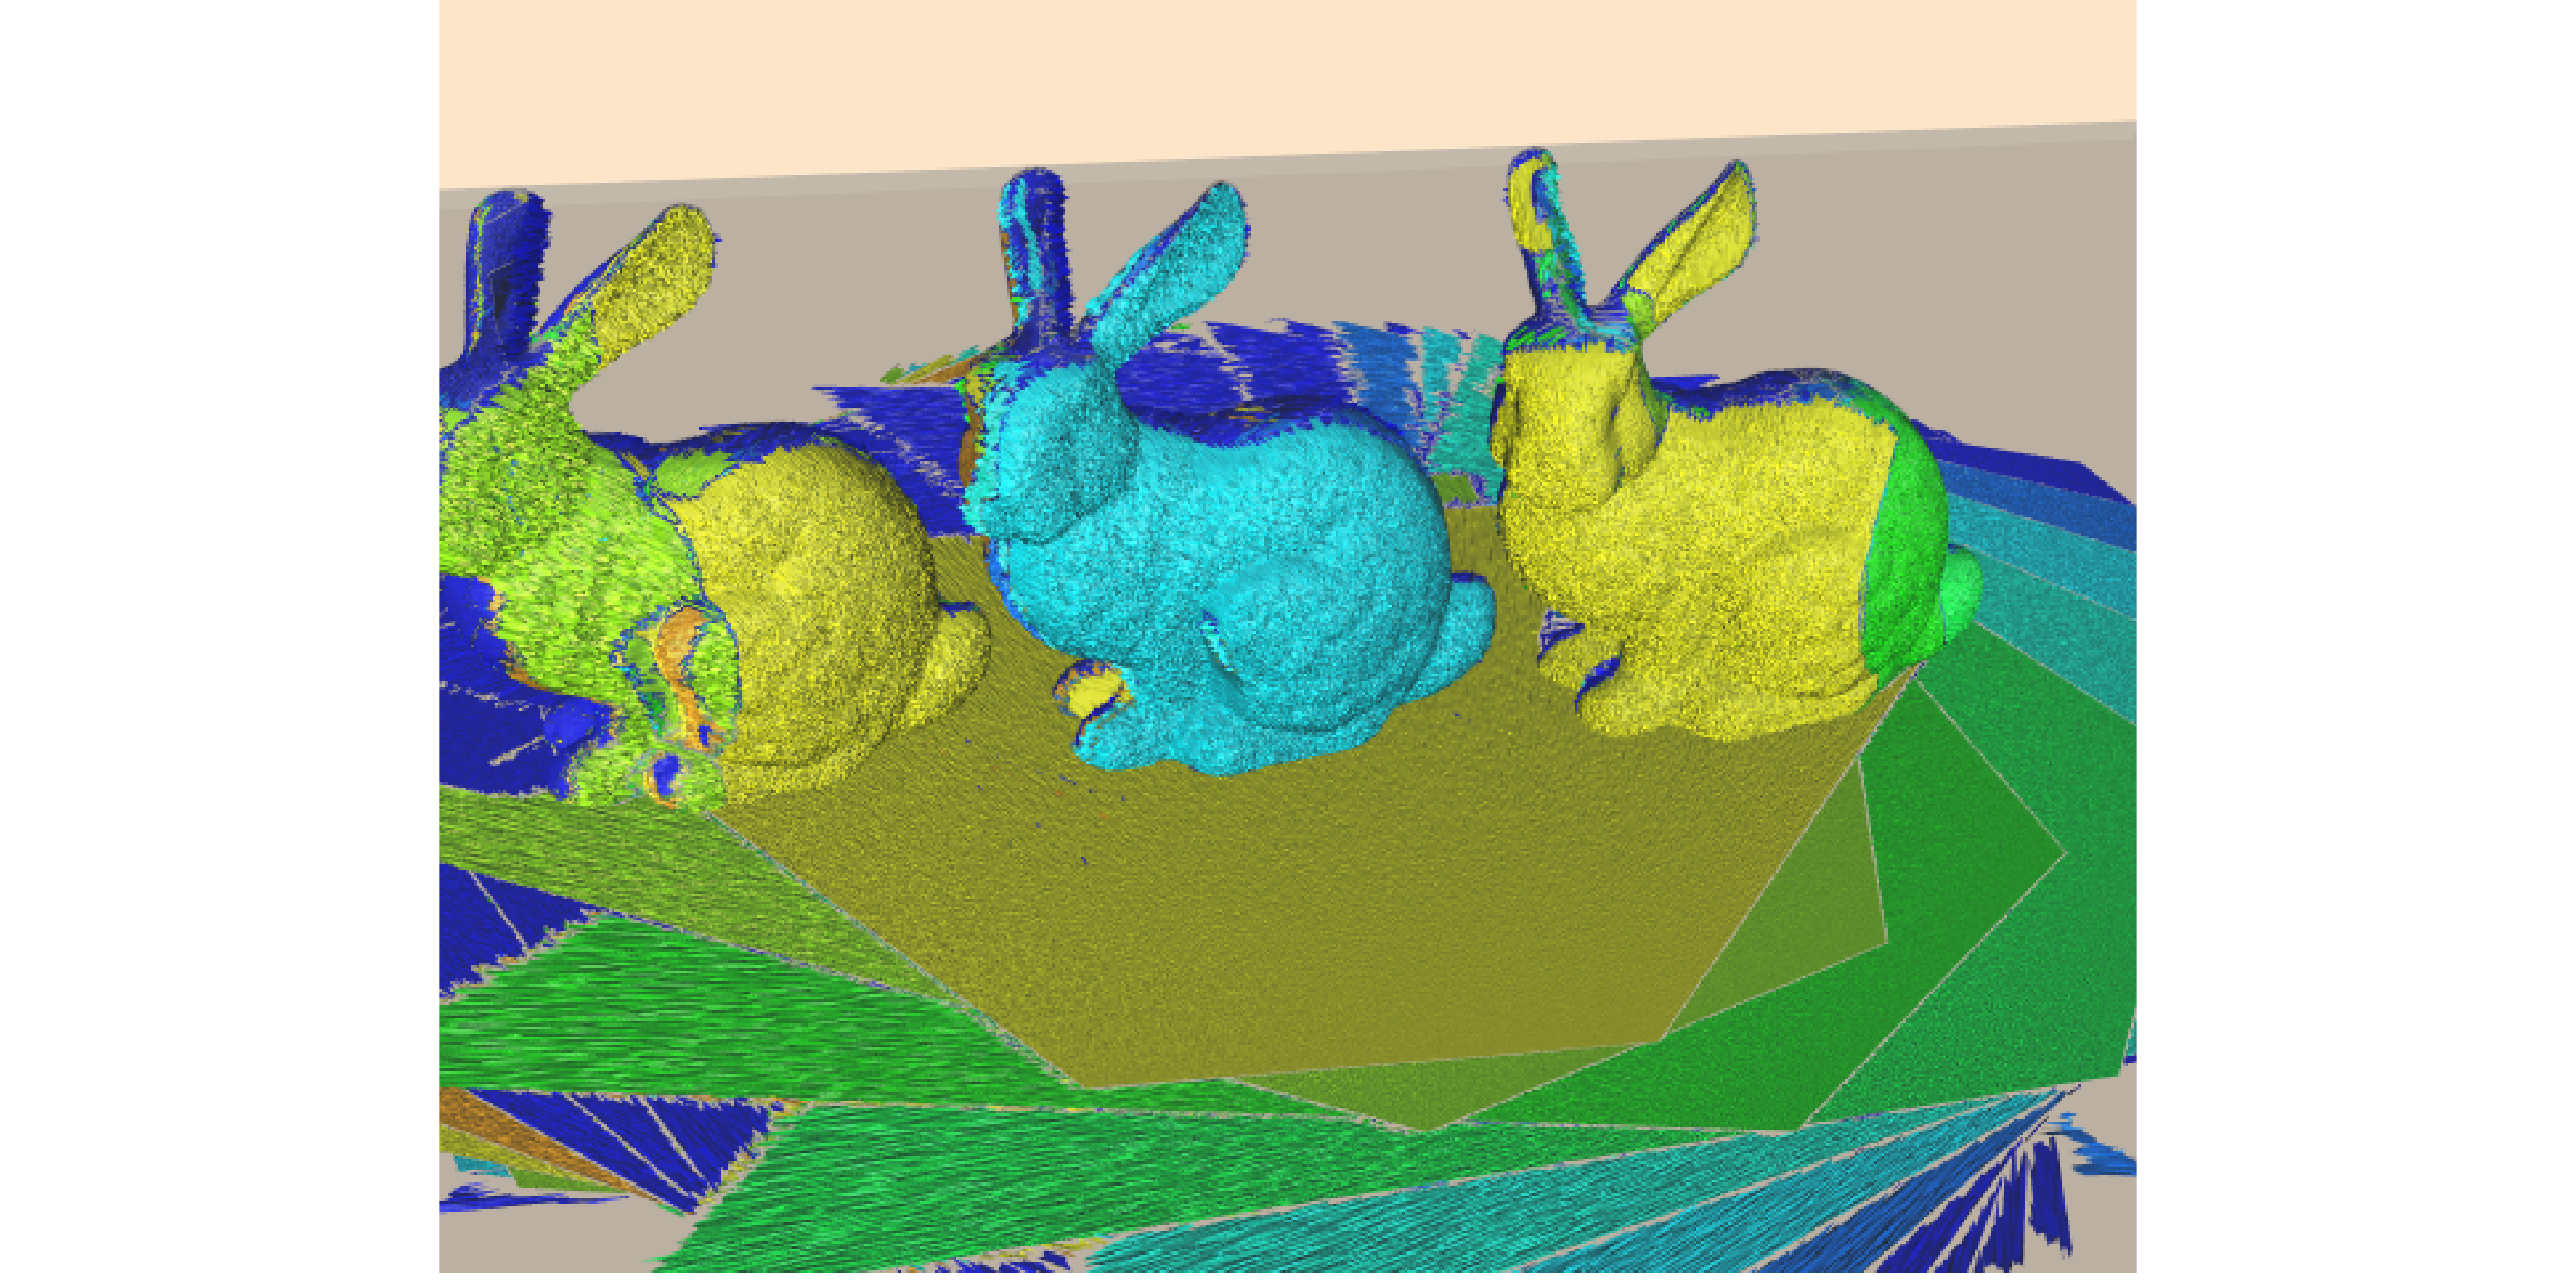
\includegraphics[width=1.2\textwidth]{../figures/results_run3_global_mesh.png}

  \note<1>{\begin{itemize}
    \item There are gaps in the mesh that occur typically along the boundaries
    of where the novel surface $S$ is appended to the global mesh $M$. This
    behavior is common for Surface Reconstruction methods as those discussed in
    Section \ref{section:surface_reconstruction}. Algorithms exist for merging
    these gaps as a post processing step such as Turk's Zippered Polygon Meshes
    \cite{Turk1994}. The aforementioned methods are typical for single object
    reconstruction. Traditional mesh-based environmental mapping algorithms
    simply append overlapping layers of mesh resulting in no gaps but a heavily
    redundant representation with a high memory cost.

    \item The mesh is noisy. This noisiness is due to the simplicity of our
    implementation's surface reconstruction method as discussed in Section
    \ref{subsection:surface_reconstruction}. Our method simply connects
    neighboring points in the point cloud without additional steps such as
    Laplacian smoothing \cite{Nealen2006}. Our reconstruction method was
    sufficient for demonstrating the usefulness of the MABDI algorithm, but
    results in a mesh with the same magnitude of noise as the sensor's simulated
    noise.
  \end{itemize}}

\end{frame}

\begin{frame}{Mesh Progression} % ______________________________________________
  \vspace{-0.15in}
  \hspace*{-12.5mm}
  \includegraphics[width=1.2\textwidth]<1>{../figures/results_run1_gm.pdf}
  \includegraphics[width=1.2\textwidth]<2>{../figures/results_run2_gm.pdf}
  \includegraphics[width=1.2\textwidth]<3>{../figures/results_run3_gm.pdf}

  \note<1>{\begin{itemize}
    \item Figure \ref{fig:gm_1} shows the resultant mesh and mesh progression for the
    first experiment. The plot highlights the major difference between MABDI
    and traditional mesh-based environmental mapping methods. Traditional methods
    would have a plot similar to that indicated by the red arrow on the graph
    because these methods have no ability to identify or remove redundant mesh
    elements. Due to MABDI's algorithmic design, MABDI has the intrinsic ability to
    identify points in the depth image corresponding to parts of the environment
    that are already known by the global mesh $M$. MABDI then simply does not use
    those points for surface reconstruction and consequently does not create
    redundant mesh elements. For this reason, the number of elements in $M$ levels
    off as the environment becomes more known.
  \end{itemize}}

  \note<2>{\begin{itemize}
    \item Figure \ref{fig:gm_2} shows us the resultant mesh after the second experiment.
    Here we can see that MABDI is reactive to the environment. In the preceding
    experiment, the environment was symmetrical. In this experiment, the environment
    is not symmetrical and we can see the effects by looking at the progression of
    the global mesh $M$. First let us note that the sensor circles the objects twice
    during the experiment and in total travels $720^{\circ}$ during the 50
    iterations. We notice when the sensor gets to $90^{\circ}$ (around iteration
    7) the number of elements begins to level off and then increases again as the
    sensor travel to $270^{\circ}$ (around iteration 19). This behavior occurs
    because the information rich perspectives of the environment occur at
    $0^{\circ}$ and $180^{\circ}$. There is less for the sensor to look at when
    viewing the environment from the sides. In this way, MABDI is reactive as the
    sensor moves to parts of the environment that are rich in information.
    Consequently, the mesh grows rapidly based on the needs of the environment.
  \end{itemize}}

  \note<3>{\begin{itemize}
    \item Figure \ref{fig:gm_3} shows us the resultant mesh after the third experiment. In
    this experiment the middle bunny was added during the twenty-sixth iteration.
    This object addition had two effects on the global mesh. First, it created a
    sudden jump in the plot as highlighted by the red circle. Second, the middle
    bunny is colored blue in the resultant mesh, signifying that it was added to $M$
    during a different iteration than the bunnies on the left and the right. Both of
    these effects indicate that MABDI was able to successfully identify the new
    bunny as novel and incorporate the bunny in to the global mesh within one
    iteration.
  \end{itemize}}
\end{frame}
